\chapter{Modelo Estrutural}
\label{sec-modelo-estrutural}
\vspace{-1cm}

O modelo conceitual estrutural visa capturar e descrever as informações (classes, associações e atributos) que o sistema deve representar para prover as funcionalidades descritas nos casos de uso especificados na Seção~\ref{sec-casos-de-uso}. 

A seguir, são apresentados os diagramas de classes de cada um dos subsistemas identificados no contexto deste projeto. Na Seção~\ref{sec-dicionario} --- Dicionário de Projeto --- são apresentadas as descrições das classes, atributos e operações presentes nos diagramas apresentados nesta seção.

\vitor{Para cada subsistema (se houverem), apresentar um diagrama de classes em uma figura separada, introduzindo a figura no texto como no exemplo da Figura~\ref{fig-modelo-estrutural-subsistema-primeiro}, abaixo. Em seguida, listar as restrições de integridade do modelo.}

A Figura~\ref{fig-modelo-estrutural-subsistema-primeiro} apresenta o diagrama de classes do subsistema 01. Para este modelo, são observadas as seguintes restrições de integridade:

\begin{enumerate}
	\item \hl{Descrever cada restrição de integridade};
	\item \hl{Ex.: um objeto da \textsf{Classe 03} não pode estar associado a si próprio}.
\end{enumerate}

\begin{figure}[h]
	\centering
	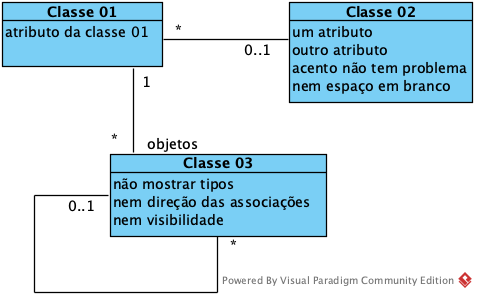
\includegraphics[width=.7\textwidth]{figuras/fig-modelo-estrutural-subsistema-primeiro.png}
	\caption{Diagrama de classes do subsistema 01.}
	\label{fig-modelo-estrutural-subsistema-primeiro}
\end{figure} 


% Replicar para outros subsistemas.
\hl{A Figura...}

\FloatBarrier
